\section{Results}\label{sec:results}

\subsection{Bayesian Optimization Convergence}\label{sec:bo_results}

Of 100 BO evaluations, 85 designs were feasible (OK) and 15 failed,
predominantly near the threshold boundary $|t| \approx 0.5$.
The unit-cell size $a$ spanned the full design range
($\num{3.0}$--$\SI{12.0}{\milli\meter}$, mean $\approx \SI{7.8}{\milli\meter}$),
and the specific surface area ranged from
$S_v \approx 770$ to $\SI{4491}{\per\meter}$.
% Fig.~\ref{fig:bo_convergence} shows the BO convergence history.

\subsection{Pareto Front and Top-5 Selection}\label{sec:pareto}

The multi-objective analysis yielded \textbf{50 Pareto-optimal points}
in the $S_v$--$\Delta P$ space (Fig.~\ref{fig:pareto}),
far exceeding the planned threshold of 15.
Five representative designs (A--E) were selected based on distinct criteria
(Table~\ref{tab:top5}).

\begin{figure}[htbp]
  \centering
  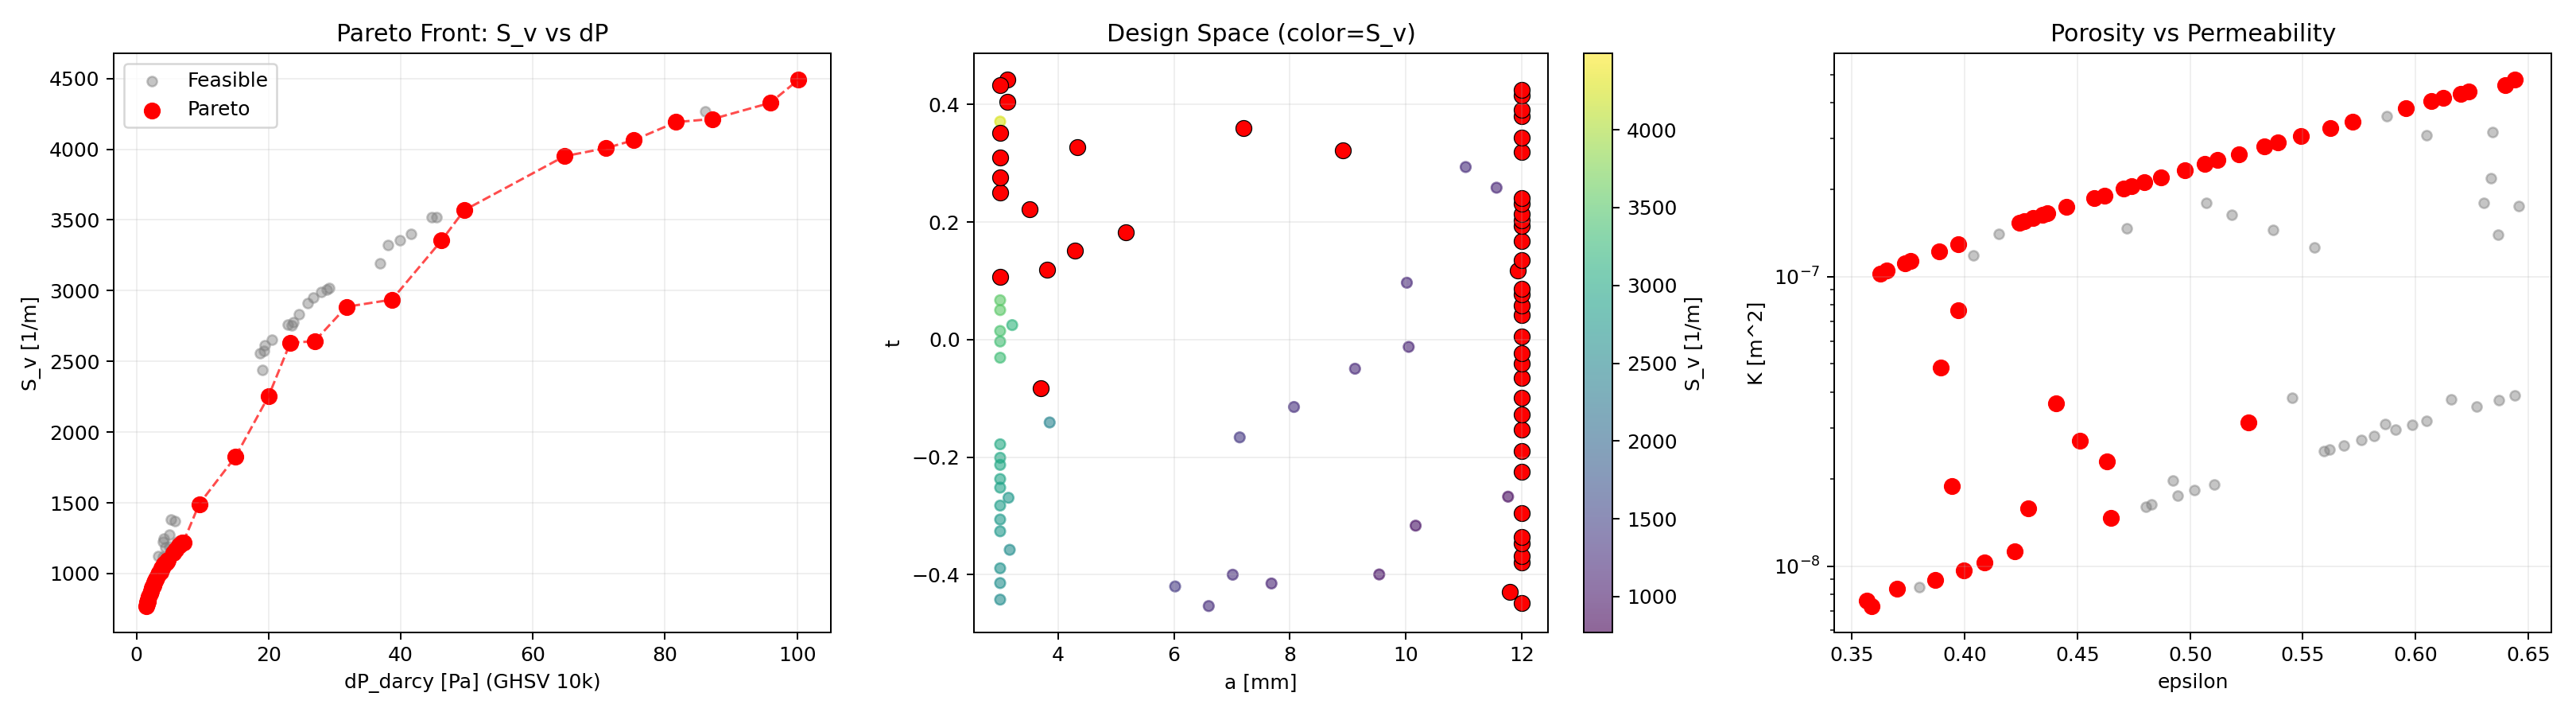
\includegraphics[width=0.85\linewidth]{figures/fig3_pareto_front.png}
  \caption{Pareto front in the $S_v$--$\Delta P$ design space.
           50 non-dominated points are identified from 85 feasible evaluations.}
  \label{fig:pareto}
\end{figure}

\begin{table}[htbp]
\caption{Top-5 selected designs from the Pareto front.}\label{tab:top5}
\centering
\begin{tabular}{@{}lccccccl@{}}
\toprule
Design & $a$ [\si{\milli\meter}] & $t$ & $\varepsilon$ &
  $S_v$ [\si{\per\meter}] & $K$ [\si{\meter\squared}] &
  $\Delta P$ [\si{\pascal}] & Criterion \\
\midrule
A & 3.00  &  0.433 & 0.359 & 4491 & \num{7.28e-9}  & 100.2 & Max $S_v$ \\
B & 12.00 & $-$0.449 & 0.644 & 770  & \num{4.79e-7}  & 1.5   & Min $\Delta P$ \\
C & 3.70  & $-$0.082 & 0.526 & 2632 & \num{3.13e-8}  & 23.3  & TOPSIS balanced \\
D & 3.00  &  0.107 & 0.465 & 3568 & \num{1.47e-8}  & 49.6  & $\varepsilon{\approx}0.5$, max $S_v$ \\
E & 5.17  &  0.183 & 0.441 & 2252 & \num{3.65e-8}  & 20.0  & Manufacturability \\
\bottomrule
\end{tabular}
\end{table}

\subsection{Flow Visualization}\label{sec:flow_vis}

Figure~\ref{fig:velocity} shows the streamwise velocity ($v_z$) contours
at the mid-plane cross-section for designs A, C, and E.
Design~A, with the smallest unit cell ($a = \SI{3}{\milli\meter}$),
exhibits the finest flow channeling pattern and strongest transverse mixing.

\begin{figure}[htbp]
  \centering
  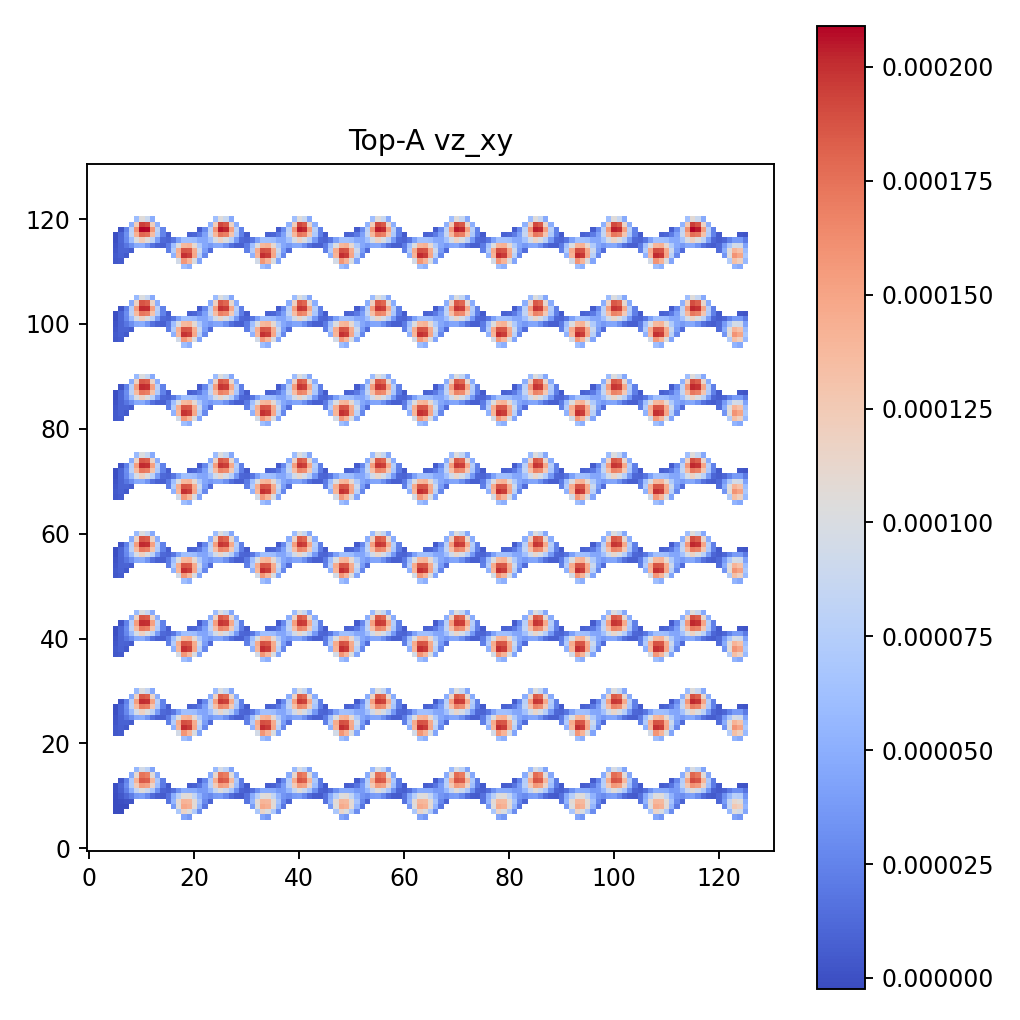
\includegraphics[width=0.32\linewidth]{figures/fig4a_vz_xy_A.png}
  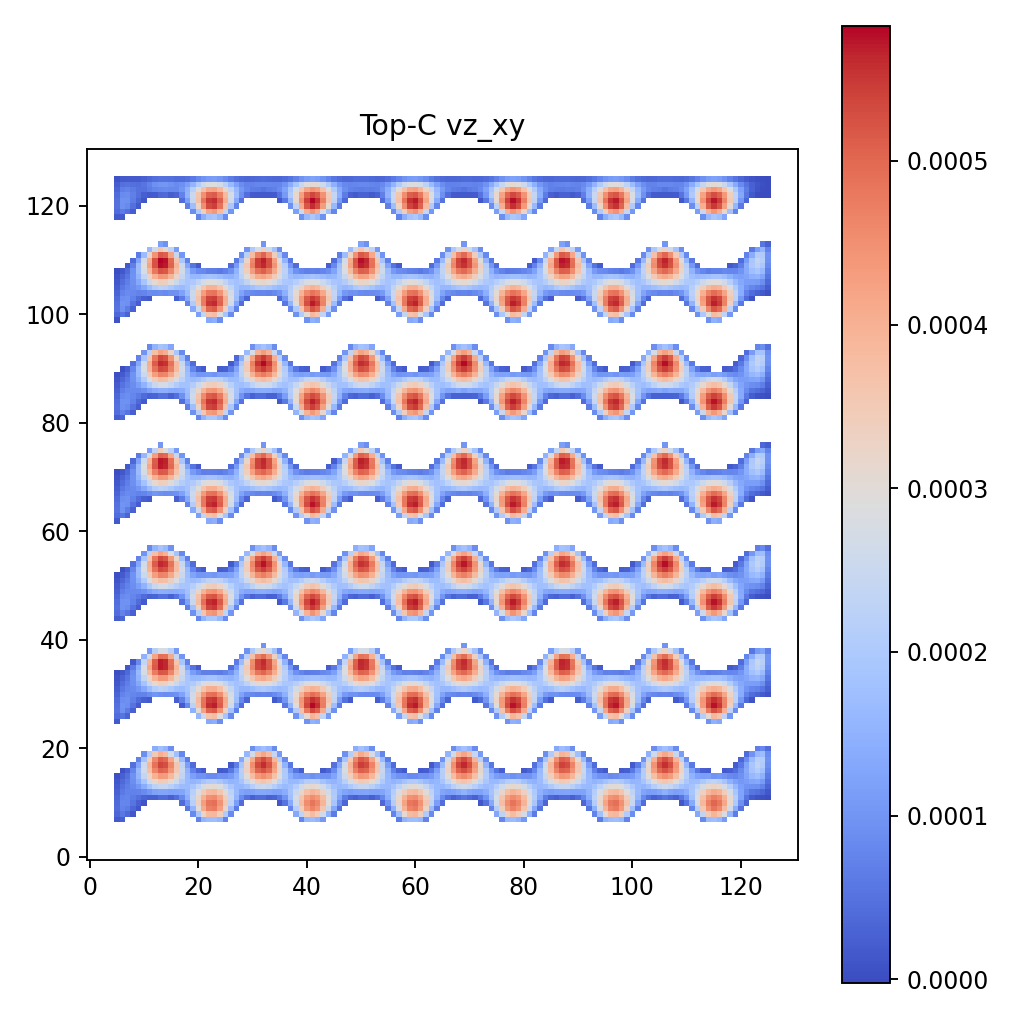
\includegraphics[width=0.32\linewidth]{figures/fig4b_vz_xy_C.png}
  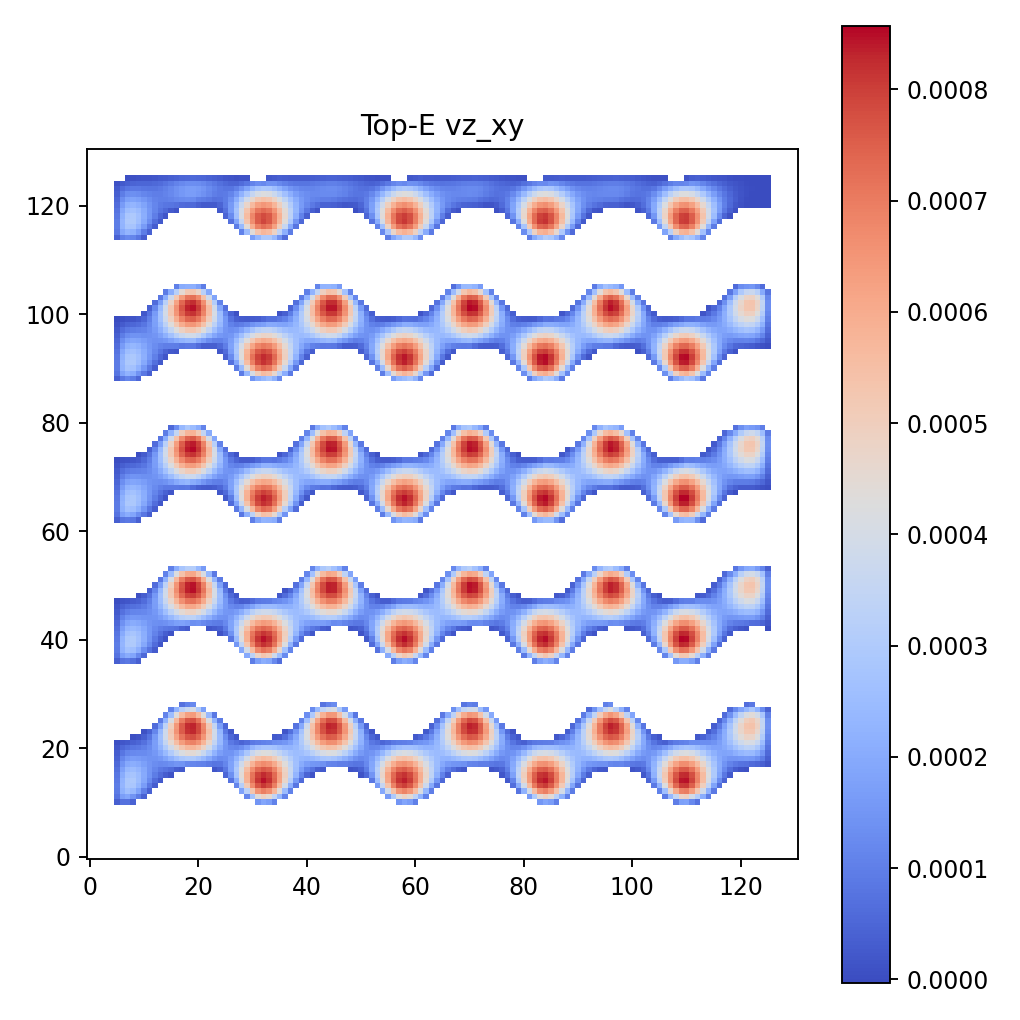
\includegraphics[width=0.32\linewidth]{figures/fig4c_vz_xy_E.png}
  \caption{Streamwise velocity $v_z$ at the mid-plane for designs
           A (left), C (center), and E (right).}
  \label{fig:velocity}
\end{figure}

\subsection{GHSV Sensitivity}\label{sec:ghsv}

Table~\ref{tab:ghsv} summarizes the Darcy-estimated pressure drop
at five GHSV conditions for all five designs.
Design~B maintains $\Delta P < \SI{10}{\pascal}$ even at
GHSV $= \SI{60000}{\per\hour}$, while design~A reaches
$\approx \SI{601}{\pascal}$ at the same condition.

\begin{table}[htbp]
\caption{Pressure drop $\Delta P$ [\si{\pascal}] at various GHSV for Top-5 designs.}\label{tab:ghsv}
\centering
\begin{tabular}{@{}lccccc@{}}
\toprule
GHSV [\si{\per\hour}] & A & B & C & D & E \\
\midrule
5\,000   & 50.1  & 0.76  & 11.7  & 24.8  & 10.0 \\
10\,000  & 100.3 & 1.52  & 23.3  & 49.6  & 20.0 \\
20\,000  & 200.5 & 3.05  & 46.6  & 99.3  & 40.0 \\
40\,000  & 400.7 & 6.09  & 93.2  & 198.4 & 79.9 \\
60\,000  & 601.2 & 9.14  & 139.8 & 297.7 & 119.9 \\
\bottomrule
\end{tabular}
\end{table}

\subsection{Forchheimer Analysis}\label{sec:forch}

Table~\ref{tab:forch} presents the Forchheimer regression results.
Designs A, C, D, and E yield $R^2 > 0.96$ with physically meaningful
inertial coefficients $\beta \sim \num{2000}$--$\SI{2900}{\per\meter}$.
Design~B, however, exhibited numerical divergence at high body-force
levels ($g_\mathrm{lbm} \ge 5{\times}10^{-4}$) due to
$\mathrm{Ma} > 0.1$, rendering its regression unreliable ($R^2 = 0.37$).

\begin{table}[htbp]
\caption{Forchheimer regression results for Top-5 designs.}\label{tab:forch}
\centering
\begin{tabular}{@{}lcccc@{}}
\toprule
Design & $K_\mathrm{Darcy}$ [\si{\meter\squared}] &
  $\beta$ [\si{\per\meter}] & $R^2$ & Remark \\
\midrule
A & \num{7.29e-9}  & 2304 & 0.966 & Reportable \\
B & \num{5.81e-7}  & ---  & 0.373 & Diverged ($\mathrm{Ma}>0.1$) \\
C & \num{3.18e-8}  & 2048 & 0.974 & Reportable \\
D & \num{1.48e-8}  & 2145 & 0.965 & Reportable \\
E & \num{3.73e-8}  & 2893 & 0.981 & Reportable \\
\bottomrule
\end{tabular}
\end{table}

\subsection{Flow Characterization}\label{sec:flow_metrics}

Table~\ref{tab:flow} summarizes the flow metrics for all five designs.
Design~A shows the highest mixing ratio (0.814), indicating strong
transverse velocity components induced by the fine gyroid structure.
All designs exhibit tortuosity $\tau > 1$, confirming flow-path
elongation relative to a straight channel.

\begin{table}[htbp]
\caption{Flow characterization metrics for Top-5 designs.}\label{tab:flow}
\centering
\begin{tabular}{@{}lcccc@{}}
\toprule
Design & Mixing ratio & Uniformity & Tortuosity $\tau$ & $\mathrm{Re}_\mathrm{pore}$ \\
\midrule
A & 0.814 & 0.694 & 1.302 & \num{6.46e-4} \\
B & 0.597 & 0.753 & 1.183 & 0.258 \\
C & 0.701 & 0.665 & 1.234 & \num{4.76e-3} \\
D & 0.739 & 0.664 & 1.258 & \num{1.63e-3} \\
E & 0.754 & 0.720 & 1.265 & \num{6.55e-3} \\
\bottomrule
\end{tabular}
\end{table}

\subsection{Numerical Reproducibility}\label{sec:reproducibility}

Five representative $(a, t)$ points were each simulated three times
with full solver reinitialization.  The coefficient of variation (CV)
of permeability $K$ was below $10^{-13}\%$ in all cases,
confirming deterministic reproducibility of the GPU-based solver.
